
The PNIPAM polymer, as it is going to be built in this tutorial, has its monomers as illustrated in Figure \ref{fig:PNIPAMPOL}.
Since the connectivity of the first and last monomers are slightly different (shown in Figure \ref{fig:PNIPAMBBs} by the asterisks), three very similar BBs were created for building PNIPAM.
%All three BBs are illustrated in Figure \ref{fig:PNIPAMBBs}.
The BBs are provided in the demo directory in pypolybuilder root, whose structure is illustrated in Figure \ref{fig:PNIPAMBBs}:
Note that the only difference between each BB is the number of carbon atoms in the backbone.

\begin{figure}
    \center
    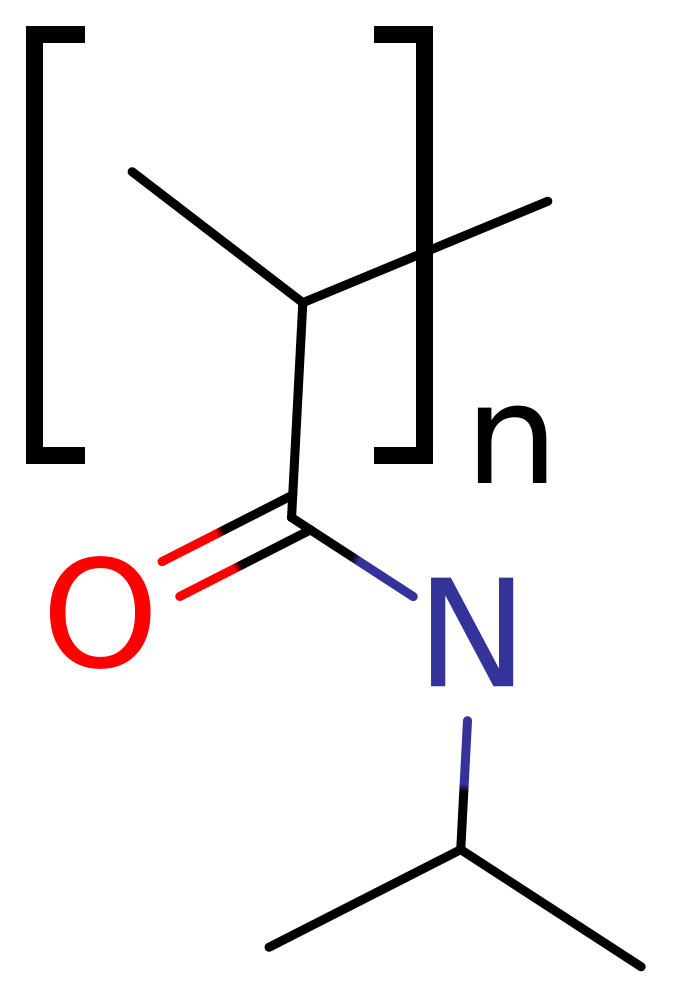
\includegraphics[width=0.3\textwidth]{PNIPAM/PNIPAMPOL.png}
    \caption{The PNIPAM polymer in the way it is built in this tutorial.}
    \label{fig:PNIPAMPOL}
\end{figure}

\begin{figure}
    \centering
    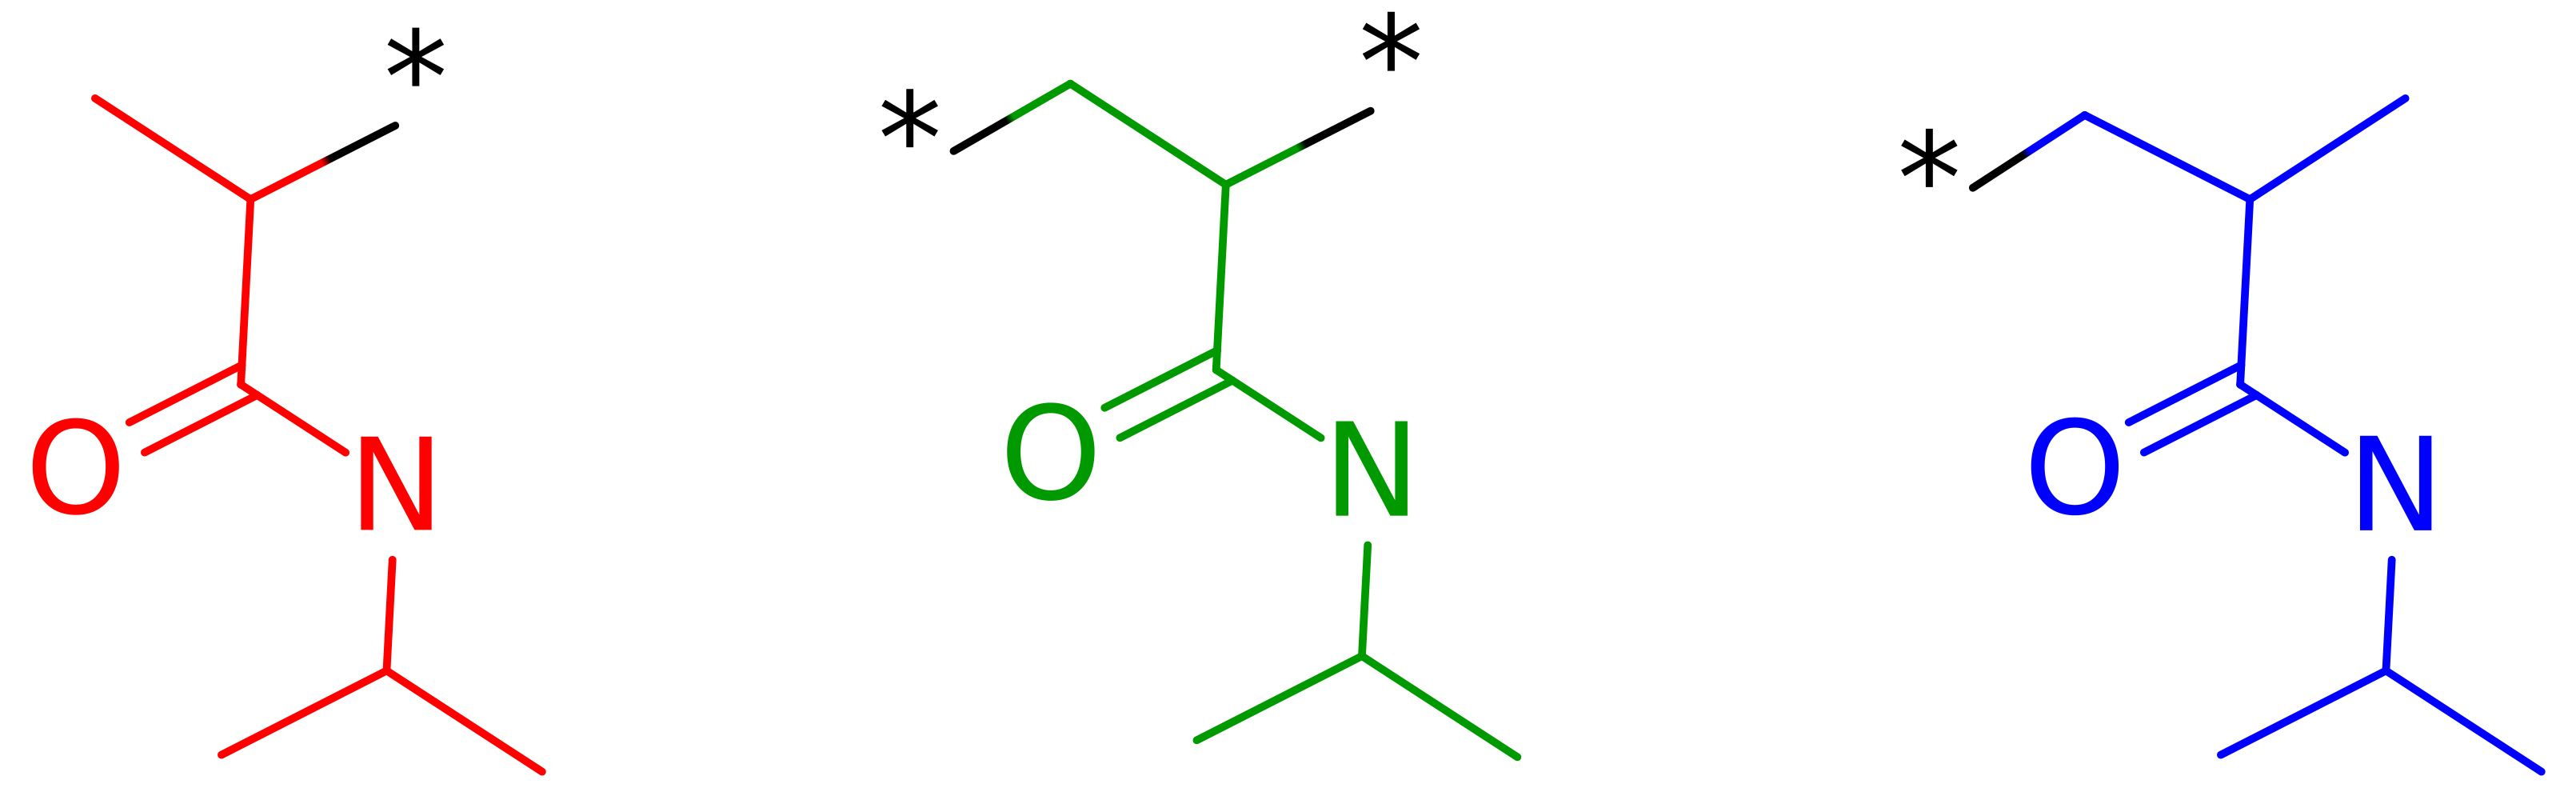
\includegraphics[width=\textwidth]{PNIPAM/PNIPAMBBs.png}
    \caption{The BBs for building PNIPAM molecules that were used in this tutorial.}
    \label{fig:PNIPAMBBs}
\end{figure}


Where \texttt{bb\_PNIP-start.itp}, \texttt{bb\_PNIP.itp}, and \texttt{bb\_PNIP-end.itp} are the first, the repeated monomer and the last BBs, respectively.
The \texttt{list\_param.itp} is the parameters file, and it should be written according to the selected force field.
The \texttt{connect.in} file is the connectivity file.
In this file, one should define the used BBs and how they are connected.
Using a smaller polymer connectivity file as an example, the \texttt{connect-5.in} file is provided with the following content:

\begin{lstlisting}
# Connectivity file to generate a PNIPAM with 5 monomers

#[ BUILDING BLOCKS ]
#BBNUM      BBNAME
  1     	PNIPS
  2     	PNIP
  3     	PNIP
  4	        PNIP
  5         PNIPE

#[ CONNECTS ]
#BBI    BBJ   IAT    JAT
 1       2     2      1
 2       3     2      1
 3       4     2      1
 4       5     2      1
\end{lstlisting}

In the field \texttt{[ BUILDING BLOCKS ]}, the user should define the names of the BBs that will be used.
Those names should agree with the \texttt{[ moleculetype ]} within each BB.
Once the BBs are defined, the field \texttt{[ CONNECTS ]} has the information about which BBs are connected (using their index numbers defined in the previous field) and which atom in each BB is used to form the connection.
For example, according to line the line 13: \texttt{1       2     2      1}, pyPolyBuilder will create a covalent bond between BBs 1 and 2 (the PNIPS and the first PNIP, respectively) using the atom 2 of the first BB, i.e., the PNIPS, and the atom 1 of the second BB, the first PNIP.
Consistently, this file contains the informations about what bonds to create in order to get the polymer built.

To build a PNIPAM with 5 monomer units, one can run the following code:

\begin{lstlisting}
python3 ../../../../__main__.py \
--bbs=bb_PNIP-start.itp,bb_PNIP.itp,bb_PNIP-end.itp \
--in=connect-5.in \
--params=list_param.itp \
--name=PNIPAM \
--output=PNIPAM.itp \
--gro=PNIPAM.gro \
--network
\end{lstlisting}

Note that the \texttt{--network} was explicitly invoked and that all the BBs are passed at once using the \texttt{--bbs} option, to be used by the \texttt{connect.in} file.

Once the optimization step is gone, the PNIPAM MTF will be ready and an initial guess for the coordinates file will be provided.
It is important to note that this guess is evaluated in vaccum and a further energy minimization stage is highly advisable to be carried out in a proper molecular dynamics package.

\begin{figure}
    \center
    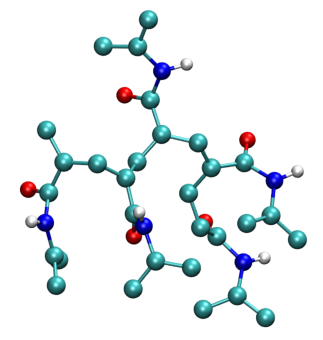
\includegraphics[width=0.5\textwidth]{PNIPAM/PNIPAMPPB.pdf}
    \caption{PNIPAM polymer with 5 monomers created by pyPolyBuilder.}
    \label{fig:PNIPAMPPB}
\end{figure}

Since pyPolyBuilder optmization steps are made in vacuum, the geometry (Figure \ref{fig:PNIPAMPPB}) may not be in the same conformation than in solution.
To carry a small simulation in water, the run directory is provided.
Copy the output from pyPolyBuilder \texttt{PNIPAM.*} to \texttt{run} and edit the \texttt{PNIPAM.sh} script to use the correct gromacs path on your machine.
By running \texttt{PNIPAM.sh}, the molecule generated by pyPolyBuilder (\texttt{PNIPAM.gro}) will be solvated in water, equilibrated, and simulated for 100 ps.
After equilibrated, PNIPAM conformation can be seen in Figure \ref{fig:PNIPAMSOL}.

\begin{figure}
    \center
    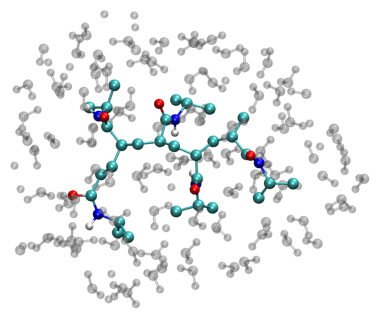
\includegraphics[width=0.5\textwidth]{PNIPAM/PNIPAMSOL.pdf}
    \caption{PNIPAM polymer with 5 monomers in water.}
    \label{fig:PNIPAMSOL}
\end{figure}

Changing the size of the polymer is not as easy as using dendrimer module.
However it is still easily doable.
Due to pyPolyBuilder philosophy, all connections are defined in a single file, hence, in order to make more connections, one only needs to edit the connectivity file.
Within this tutorial directory, two connectivity files are provided: \texttt{connect-5.in} and \texttt{connect.in}.
The former connects 5 monomers of the PNIPAM polymer, while the latter uses the same three BBs to build a 30-mer.
Using the \texttt{connect.in} as the connectivity file, one can simply run the code:

\begin{lstlisting}
python3 ../../../../__main__.py \
--bbs=bb_PNIP-start.itp,bb_PNIP.itp,bb_PNIP-end.itp \
--in=connect.in \
--params=list_param.itp \
--name=PNIPAM \
--output=PNIPAM.itp \
--gro=PNIPAM.gro \
--network
\end{lstlisting}

That is very similar to the previous one.
In fact, only the \texttt{--in} option was changed.
Both built polymers can be seen in Figure \ref{fig:PNIPAMSIZE}.

\begin{figure}
    \center
    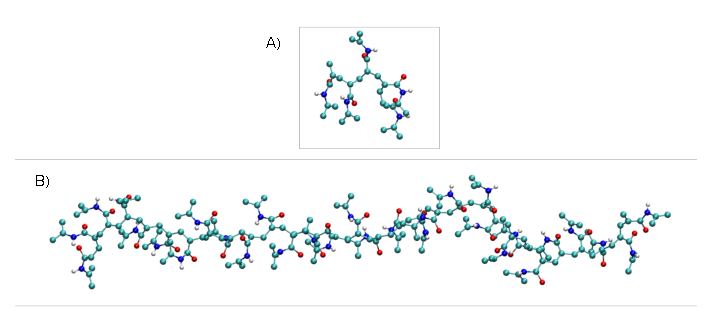
\includegraphics[width=\textwidth]{PNIPAM/PNIPAMSIZE.pdf}
    \caption{PNIPAM polymers created by pyPolyBuilder.
    These two polymers were used to illustrate the simplicity of using pyPolyBuilder for varying the size of the created molecule. A) is a PNIPAM with only 5 monomers while B) is a PNIPAM with 30 monomers.
    The same BBs were used for both polymers.}
    \label{fig:PNIPAMSIZE}
\end{figure}